\chapter{Design of Mobile Platform}
\label{ch_3:KPI}
%The % Comment the below command to supress the random text
%\lipsum[3-20]
% % % % % % % % % % % % % % % % % % % % % % % % % % % % % % % % %

Most of the mobile robots presented in literature uses differential wheel drive  with passive castor, as in \cite{yamamoto1992coordinating}, \cite{rajendran2004} and \cite{saha1989kinematics}. The other  common methods for locomotion of mobile robots are the omnidirectional wheels  \cite{pin1994new} and \cite{salih2006designing}, and tracked wheel system \cite{suthakorn2009design} and \cite{guarnieri2004development}. According  to  Nagatani \cite{nagatani2000improvement},  a  vehicle  with  Mecanum  wheels  is  susceptible  to slippage and same is the case for tracked vehicle, which are inherently skid steered. The slippage of the wheels prevents the most popular dead-reckoning method using rotary shaft  encoders   from  being  performed  well. This chapter   discusses the  design methodology of a novel mobile manipulator based on environmental requirements. We also  highlight the advantage of the Davis steering mechanism over castor wheels  or other steering methods from the perspective of this mobile manipulator.   The Davis steering system modifies the heading of  front wheels in a way that, at low speeds, all the wheels are in pure rolling without lateral sliding \cite{wong2008theory}.  
%The kinematics and control of such systems are discussed in \cite{d1992dynamic} and references therein but no detail design is presented.  


\section{Design Overview}
 The objective of a  mobile robot under consideration is to navigate inside the cyclotron vault and collect radiation intensity data at all the required points decided by the operator. Data is to be collected not only at different planer locations of the floor but also at varying height from the floor. To cater to this operational requirement, a mobile platform with a vertically extendable manipulating arm was developed as shown in  Figures \ref{fig:robo3Dmodel} and \ref{fig:roboActual}. Together, they are   referred henceforth as mobile-manipulator. The 3-D model of the mobile-manipulator with its major subsystems are shown in Figure \ref{fig:robo3Dmodel}, whereas  and the actual   system  is shown in Figure  \ref{fig:roboActual}. 

 The environmental condition required that the vehicle be either  autonomous or teleoperated. To keep the complexity low it was decided to have wireless teleoperated   navigation and control. This gives an  operator full flexibility to drive  and control the system from a remote station  using  visual  feedback provided by the on board camera. The key parameters of the mobile manipulator are listed in  Table \ref{tb:specifications}.


 \begin{figure}
 	\centering
 	\begin{minipage}{.5\textwidth}
 		\centering
 		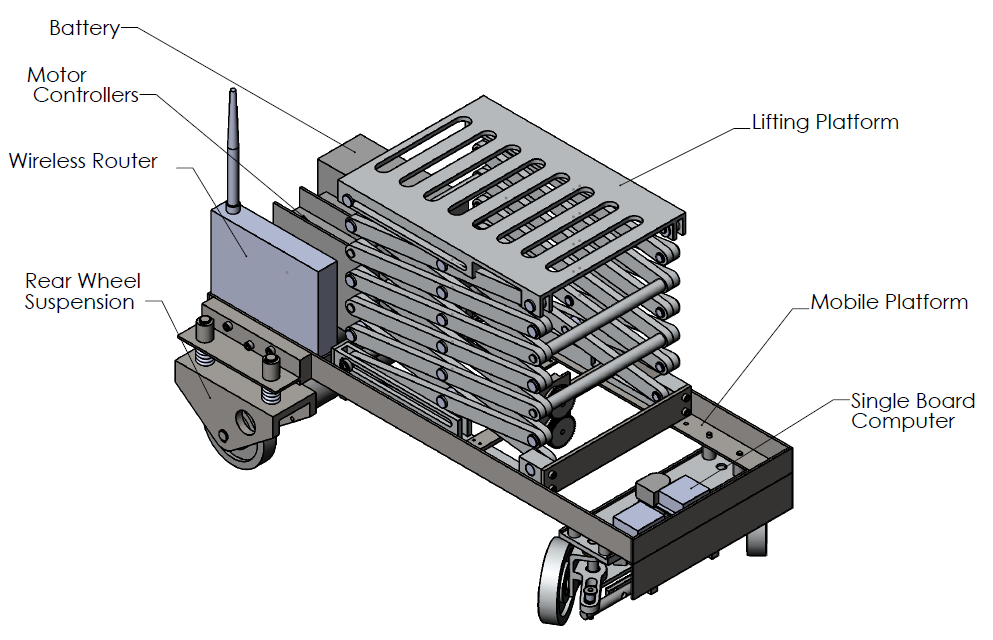
\includegraphics[height=5cm,keepaspectratio]{Chapter3/fig/robo3Dmodel}
 		\captionof{figure}{3-D Model of the mobile manipulator}
 		\label{fig:robo3Dmodel}
 	\end{minipage}%
 	\begin{minipage}{.5\textwidth}
 		\centering
 		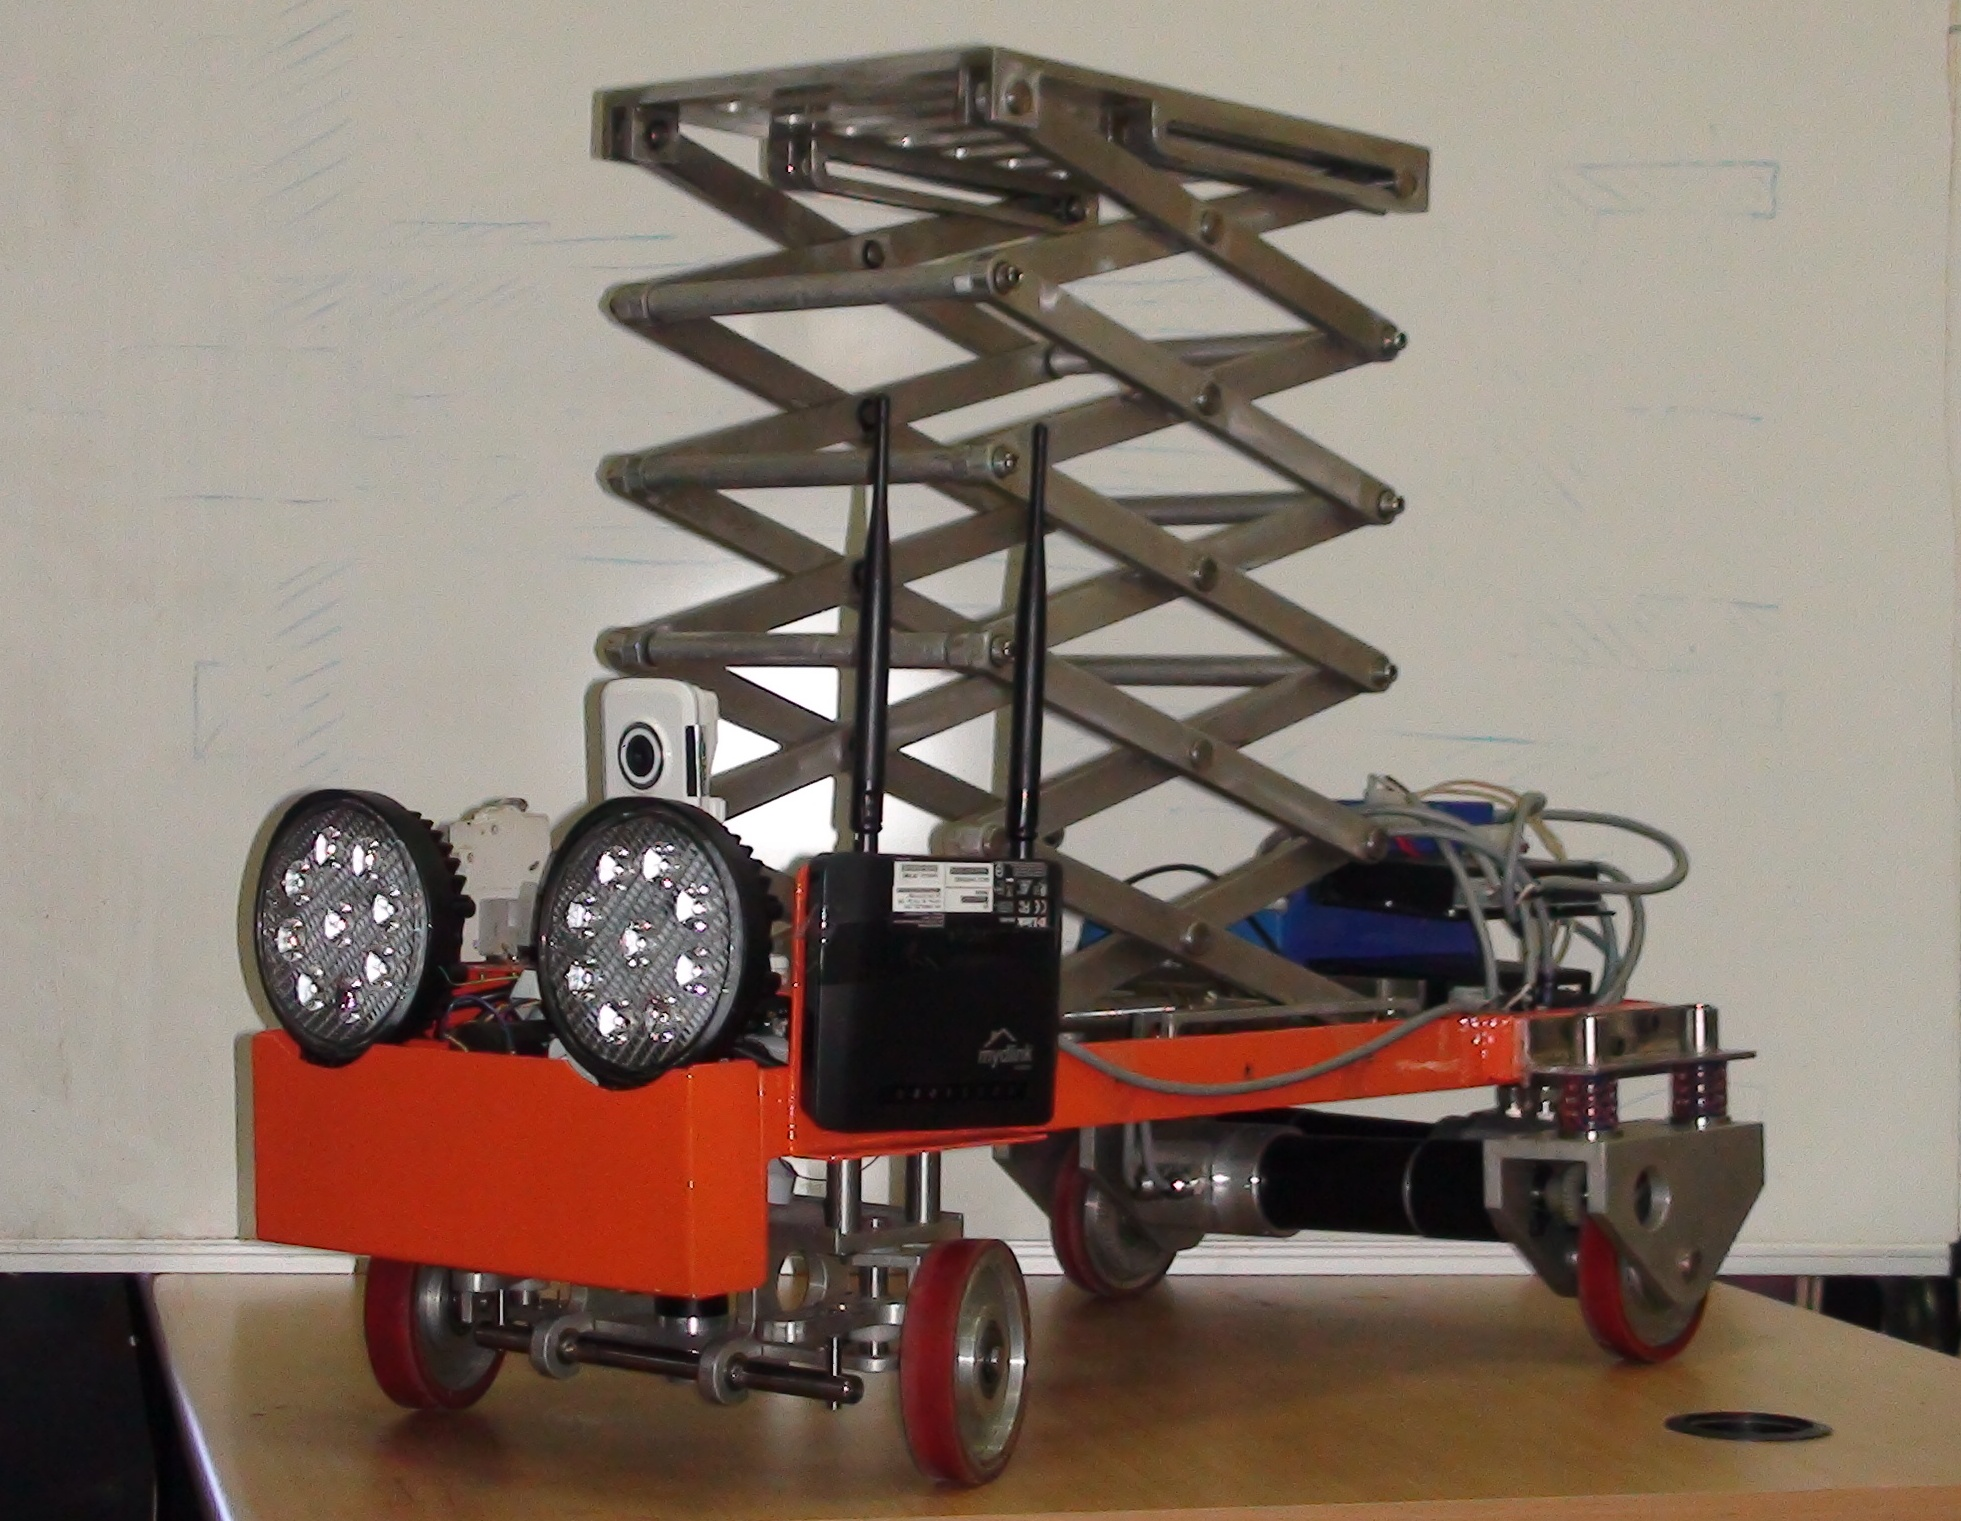
\includegraphics[width=.8\linewidth,height=5cm,keepaspectratio]{Chapter3/fig/roboActual}
 		\captionof{figure}{Photograph of the actual System}
 		\label{fig:roboActual}
 	\end{minipage}
 \end{figure}

%
\begin{table}[!htbp]
	\caption{Key parameters and specifications of the mobile manipulator.}
	\label{tb:specifications}
	\centering
	\begin{tabular}{l l l}
		\hline
		
		%\emph{Parameter}  & \emph{Example} & \emph{Font size and style} \\
		%\hline
		Weight  & 70 Kg & without payload \\ 
		Payload & 10 Kg &---\\
		Footprint & 700 mm $\times$  400 mm & - \\
		Height Collapsed & 500 mm  & Along  Z-Axis\\
		Height Extended & 1500 mm & Along  Z-Axis  \\
		Steering mechanism & Davis Steering & --\\
		Turning radius & 415 mm & - \\
		Ground clarence & 45 mm & --\\
		Maximum traction speed & 2 m/min & On flat terrain \\
		Ramp climb angle & $30^\circ $ & Checkerboard surface\\
		\hline
	\end{tabular}
\end{table}

The mobile-manipulator has a footprint of 700 mm x 400 mm  based on the narrow passage through which the system  has to negotiate. These passages are formed inside the vault area by the pipelines and  structural supports of the cyclotron and its associated equipment.  Two DC motors,with speed servo controller,  provide the traction to each rear wheels. The two front wheels are  inter-connected with a Davis steering mechanism \cite{TOMBook}. A scissor mechanism provides the vertical  motion of the detector that is mounted on the manipulating arm.

 In order to keep the self weight of the system small all the  structural parts are made of aluminum alloy AL6061, apart from the base frame. Stainless Steel (SS304)  angle sections was used for the base frame, which give it  excellent strength to weight ratio. 

\section{Design of the Traction System}
Traction is provided by the two rear wheels driven independently. This makes the system over actuated. A mechanical differential connecting the two rear wheels, as used in cars,  would overcome this. It was not proposed to do so as the proposed vehicle is planned to be teleoperated in a environment inaccessible to humans. This calls for a single-failure-safe design. The proposed design gives two major advantages. 
Firstly, in case  one of the wheel loosing contact with the ground due to  overhang in small pits or while over an obstacle, the mechanical differential system would keep supplying power to the free hanging wheel. The system will hence get stuck, maybe in an unrecoverable location. This situation is avoided in the present design as the motor having traction can be independently powered, to move the vehicle.  
Secondly, using the proposed design, in case of one  actuator failure, either the traction or the steering motor, still the vehicle can be manoeuvred to a  safe location, albeit with dragging of the wheel with failed actuator.

    Each wheel is driven by a  Maxon DC RE50 200W Motor through a 26:1 reduction gearbox. The motors are mounted at an offset to the wheel axis for increased ground clearance, as shown in Figure \ref{fig:tractionDrive}. Spring suspension is provided at each wheel to ensure sufficient contact force on uneven  ground. The diameter of the wheel is 100 mm $(D_w)$, which is sufficient to ride over obstacle of height 20 mm (Max). They are made of Aluminum alloy-6061 with 5mm thick molded polyurethane (PU) liner. The PU liner provides large traction on cement flooring while being resistance to wear.

  The load distribution was optimized to generate maximum normal reaction, $F_n$,  at the rear wheels without overturning while moving up the ramp of $30^o$. Maximizing rear wheel reaction by increasing  "b" as per Equation \ref{eqn:loadratio} ensures increased traction, $F_T=\mu F_N$ ($\mu$ is the coefficient of friction), but at the same time decreases the stability margin indicated by "X" in Figure \ref{fig:loadDistribution}. The static moment and force balance yield
\begin{equation}
\label{eqn:loadratio}
F_{N2}=\frac{b}{a}F_{N1}, \quad F_{N1}+F_{N2}=mg\cos\theta
\end{equation}

The stability margin $X$ as shoen in Figure \ref{fig:roboActual} was fixed as $30mm$ so as to achieve  maximum acceleration of $0.144g$  over the ramp of $30^o$ without overturning. This was done based on the condition of dynamic stability given by
\begin{equation}
\label{eqn:overturn}
mgb\cos\theta=(mg\sin\theta+ma)z_{cg}, \quad \Rightarrow g(\frac{b}{z_{cg}}\cos\theta-\sin\theta)=a
\end{equation}


Where 
\begin{itemize}
\item[] $F_{N1}$, $F_{N2}$ are normal reaction on the front and rear wheels.
\item[] a and b are the distance of the vehicle cg from the rear and front wheels.
\item [] $Z_{cg}$ is the height of the cg from the  plane containing the contact point of the wheels.
\item [] $m$ is mass of the vehicle.
\item [] $g$ is acceleration due to gravity.
\item[] $\theta$ is the inclination of the traction surface from horizontal.
\end{itemize}


 
\begin{figure}
 	\centering
 	\begin{minipage}{.5\textwidth}
 		\centering
 		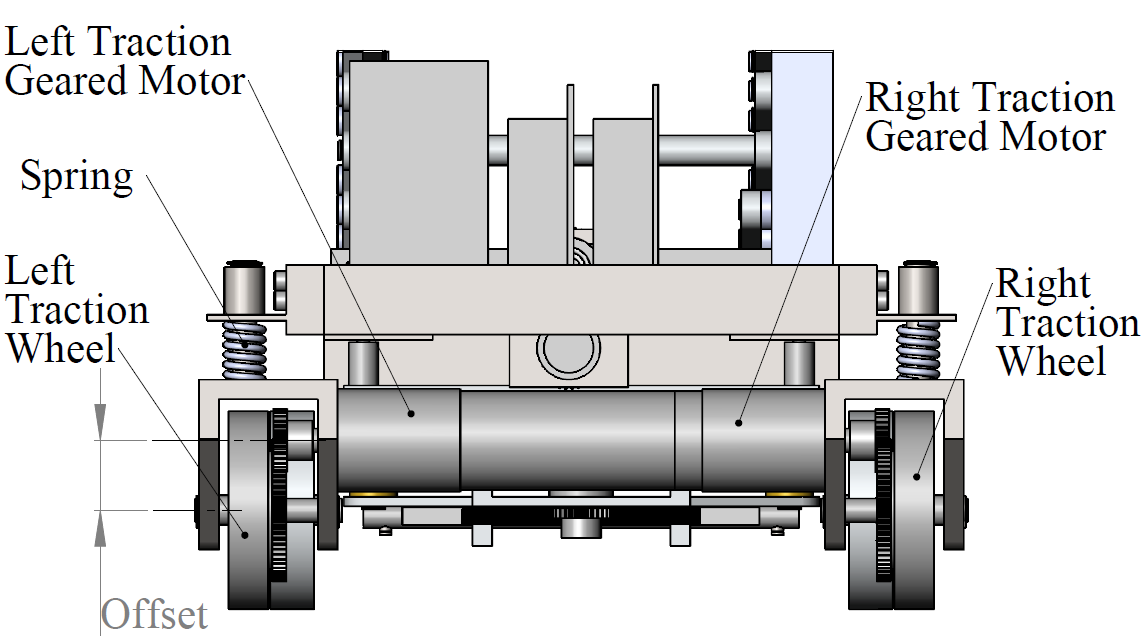
\includegraphics[width=.9\linewidth,height=4.5cm,keepaspectratio]{Chapter3/fig/WheelOffset}
 		\captionof{figure}{Rear Suspension}
 		\label{fig:tractionDrive}
 	\end{minipage}%
 	\begin{minipage}{.5\textwidth}
 		\centering
 		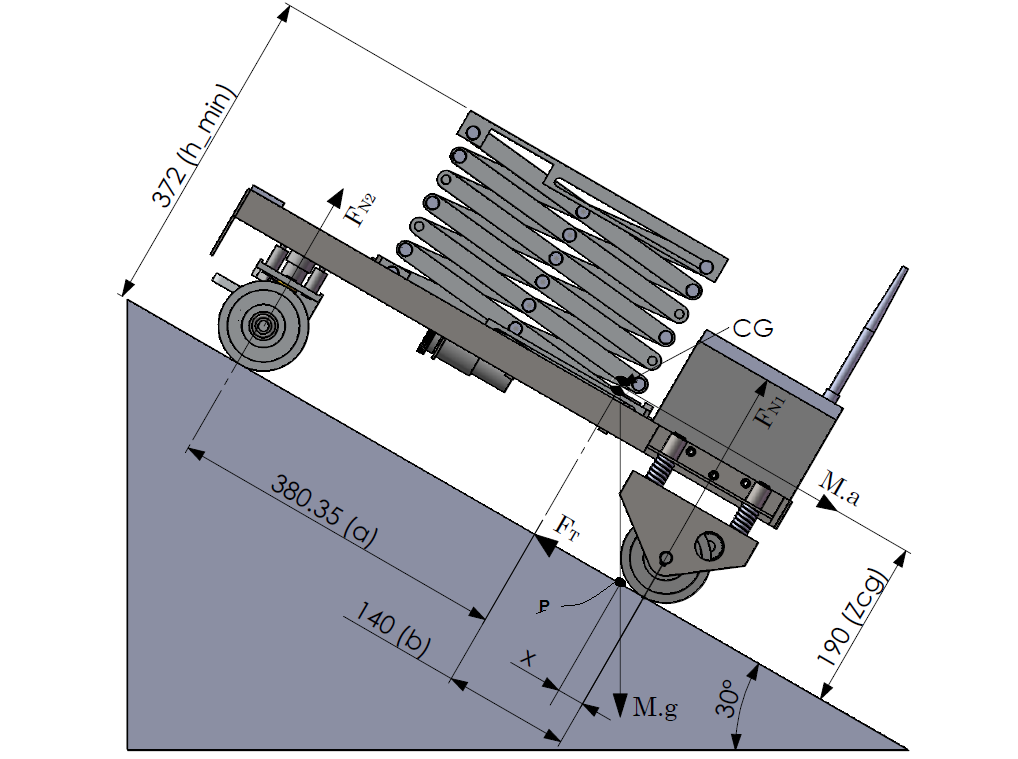
\includegraphics[height=4.5cm,keepaspectratio]{Chapter3/fig/loadDist}
 		\captionof{figure}{Mobile Manipulator on slope}
 		\label{fig:loadDistribution}
 	\end{minipage}
 \end{figure}
 \subsection {Selection of Motor and Gearbox}
 The torque requirement for each rear wheel was calculated based on the static moment balance with the assumption that each rear wheel shares equal load and the total suspended weight is 80 Kg. From the freebody diagram (Figure   \ref{fig:loadDistribution}), using moment and force balance  we get the following:
\begin{equation}
\label{eqn:t1}
F_{N1}=\frac{a M \cos \theta}{a+b-\mu Z_{cg}} , \quad \quad
F_T=\mu F_{N1}
\end{equation}
In order to estimate the traction motor size, we take worst case scenario of $\theta=30^o$ and $\mu =0.3$. This leads to
\begin{equation*}
F_{N1}=66 Kg, \quad\quad F_T=0.3*66 \approx 20Kg
\end{equation*}
 Since the traction is provided by the two rear wheels, the torque required per wheel $(T_w)$ is given by
\begin{eqnarray}
T_w=(F_T/2)(D_w/2)= (20/2)*50=500 Kg-mm \simeq 5 Nm
\end{eqnarray}
The motor torque $T_M$, required based on the assumption of factor of safety, $FS=1.5$ is
\begin{equation}
T_M=(FS)*T_w=1.5*5 =7.5 \simeq 8Nm
\end{equation}
 Assuming the maximum speed, $V_{ramp}=1m/s$, of the mobile manipulator over a ramp, the required power, $P_M$, of the traction motor is calculated as,
 \begin{equation}
 \begin{aligned}
\omega_w&=V_{ramp}/(D_w/2) \simeq 200rpm\\
P_m&=\omega_w T_m=20*8=160W
 \end{aligned}
 \end{equation}
 The nearest Maxon motor available as per the catalogue \cite{catMaxon} is 200W,  RE50-370354 motor.  The nominal speed, $N_s$ is 5680rpm. Therefore, the  gearing  ratio required is, $N_s/\omega_w=5680/200 \simeq 28.4$. The nearest gear box available  is of ratio $26:1$, which was chosen. 

\section{Design of Steering System }
The design objective of a steering system should ensure rolling motion of all the  wheels during every possible manurers of the mobile robot. This is important to reduce the friction drag due to sliding motion which reduces the energy efficiency of the mobile robot. In case of four wheeled vehicle with rear wheels fixed and front wheels steered the condition is  shown in Figure \ref{fig:steerCond},  referred in some literature as Ackerman steering conduction.   

This mobile manipulator uses Davis steering mechanism,  Figure \ref{fig:davis},  on the front wheels. Caster wheels  were not used as they tend to align with  obstacles and thus get stuck. On the  other hand tracked wheels have excellent rough terrain capabilities, but is power intensive due to skid steering. another option was to use   Omnidirectional wheels, which need complex controller for coordination and an extra actuator. Moreover, the operation are are in general not clean of loose small objects, which may get stuck in between the free rollers of the omnidirectional wheels. This will reduce the efficiency of the vehicle.  

\begin{figure}
 	\centering
	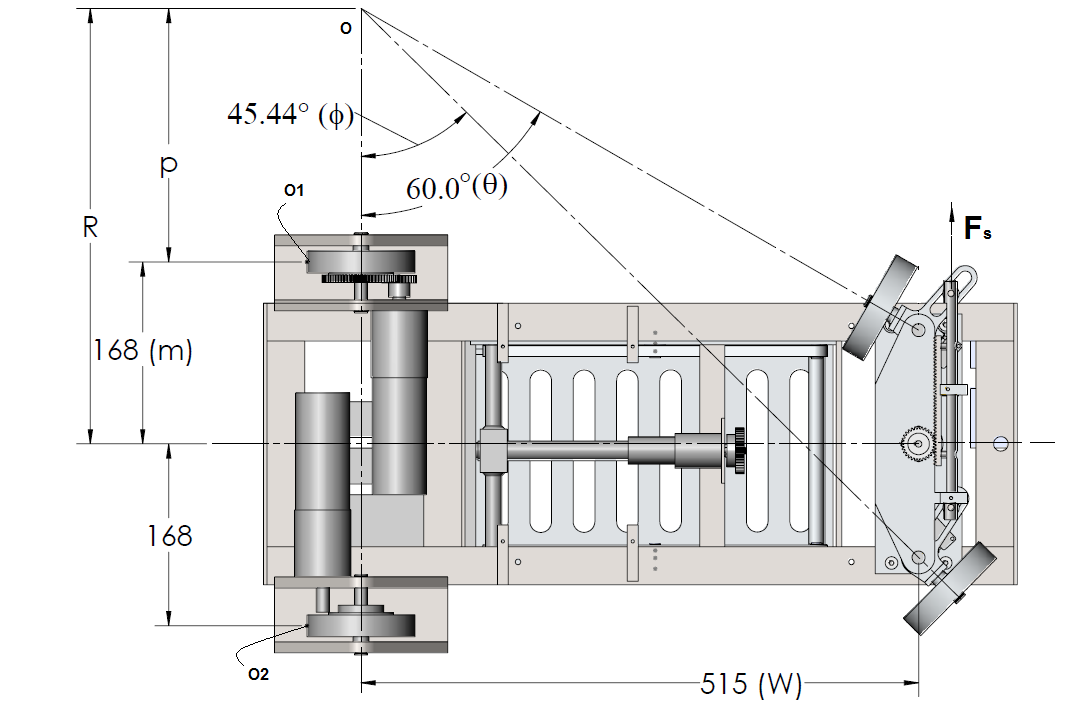
\includegraphics[width=\linewidth,keepaspectratio]{Chapter3/fig/steerringCondition}
	\captionof{figure}{Ackerman Steering Condition }
	\label{fig:steerCond} 
\end{figure} 
 

Davis mechanism was chosen over Ackerman steering gear as it satisfies the steering condition given by  Equation \ref{eqn:Acker}, which ensures pure rolling of all  wheels over the entire steering range. This makes the system suitable for passive wheel odometry and energy efficient.  The mechanism being positively driven by position controlled servo motor does not align with the obstacles and thus are able to crossover it. The dimensions of the links used in the steering mechanism is given in Figure \ref{fig:davis}, and are based on the Ackerman steering law given below:
\begin{equation}
\label{eqn:Acker}
\cot\phi-\cot\theta=a/w, \quad  \frac{2b}{h}=\frac{a}{w}
\end{equation}
Where $a$ and $b$ is limited by the over all size of the vehicle, discussed earlier.

\subsection{Minimum Turning Radius}
The mechanical construction of this steering mechanism limits the steering angle. This in turn limits the minimum radius the vehicle can negotiate.
Figure \ref{fig:steerCond} shows the extreme values of $\phi$ and $ \theta$, one side of the steering limits. The \textbf{ turning radius } $R$ for a given steer angle $\theta$  is calculated  by the geometry of Figure  \ref{fig:davis} as
\begin{equation*}
\tan\theta =\frac{w}{P+m-\frac{a}{2}} \quad \text{and} \quad R=m+p
\end{equation*}
Substituting $R$ and rearranging the above equation, we get 
\begin{equation}
\label{eqn:turningRadius}
R(\theta)=\frac{a}{2}+w\cot\theta
\end{equation}
The extreme value of $\theta=60.$ as shown in Figure \ref{fig:steerCond}, this gives the \textit{minimum turning radius } $R_{min}$ as
\begin{equation*}
R_{min}=\frac{210}{2}+515 \times cot(60^o)=402mm
\end{equation*}

\begin{figure}
	\centering
	\begin{minipage}{.5\textwidth}
		\centering
		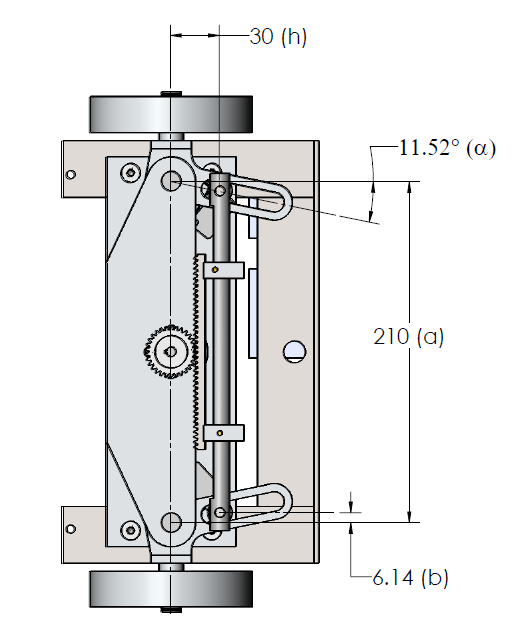
\includegraphics[width=\linewidth,height=5cm,keepaspectratio]{Chapter3/fig/davis}
		\captionof{figure}{Davis Steering Gear}
		\label{fig:davis}
	\end{minipage}%
	\begin{minipage}{.5\textwidth}
		\centering
		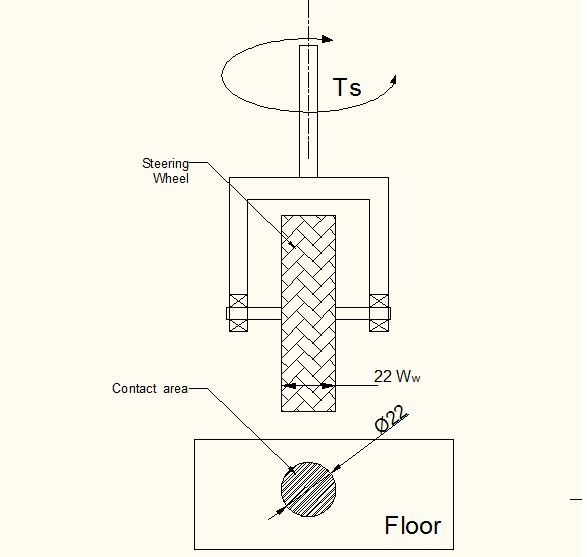
\includegraphics[width=\linewidth,height=5cm,keepaspectratio]{Chapter3/fig/steerTorqCal}
		\captionof{figure}{Steer Torque}
		\label{fig:steerTorq}
	\end{minipage}	
\end{figure} 

\subsection{Calculation of Steering Torque}
The torque required to steer the front wheel is estimated based on a simplified assumption that the wheel deforms under normal load and the contact area thus generated is  circular in shape with diameter that of the wheel width, $W_w$, as shown in Figure \ref{fig:steerTorq}. 
In order to estimate the normal reaction on each wheel, we assume that the total weight of 80kg is equally shared by the four wheels. 
Therefore, $N_s=80/4=20Kg$. Next, the uniform pressure formula used for  brakes/clutches design was applied to find the resistance  torque $T_s$, between the ground and the wheel i.e, 
\begin{equation}
\label{eqn:brake}
T_s=\frac{N_s\mu}{3}W_w= 0.4Nm
\end{equation}  
The resistance torque, $T_s$, of  both the wheels  are balanced by the force $F_s$ acting on the rack as shown in Figure \ref{fig:davis}. The rack is coupled to the steering motor by a pinion of diameter, $D_p=40mm$. The motor  torque, $T_{m_s}$  in Equation  \ref{eqn:SteerTq} is calculated with a  high factor of safety, $FS=3$. This is because $T_S$ is estimated  based on a simplified model of brake design. The power, $P_{m_s}$ of the steering motor based on  torque $T_{m_s}$ and the steering speed $\omega_s$ of 100rpm is 
\begin{equation}
\begin{aligned}
\label{eqn:SteerTq}
T_{m_s}=(FS)\frac{2T_s}{h}\frac{D_p}{2}=1.6Nm \quad \text{and}\quad P_{m_s}=T_{m_s}*\omega_s=17W
\end{aligned}
\end{equation} 

Based on the above specifications, a 20W, RE25 DC motor of Maxon  make and a gear box  GP32 of ratio 159:1 was chosen for the steering mechanism. 
 
\section{Design of Scissor Mechanism for Manipulating Arm}
 The manipulating arm  was designed to move  up to a height of 1.5m from the floor level. This motion was generated using  a scissor mechanism, as shown in Figure \ref{fig:scissor}. The scissor mechanism has two major advantages over other lifting methods such as telescopic pillar, etc.  First, the  ratio of height in extended and collapsed condition is very large. In our case it is $3:1$. Second, the self weight of the mechanism is less as it is made of rectangular links.

The scissor mechanism, Figure \ref{fig:scissor}, has 6 stages, where one "X" denotes one stage. 
\begin{figure}
	\centering
	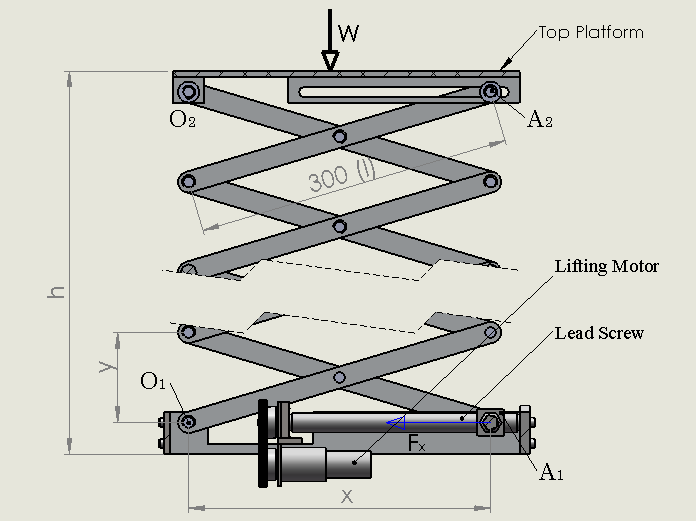
\includegraphics[width=\linewidth,keepaspectratio]{Chapter3/fig/scissor}
	\captionof{figure}{Scissor Mechanism}
	\label{fig:scissor}
\end{figure}
The Scissor is connected to the top platform by a pivot joint $O_2$ and a prismatic joint $ A_2$.
 This is coupled to the base frame by pivot joint $O_1$ and a prismatic joint $A_1$. The linear actuation of joint $A_1$ is provided by a lead screw of pitch ($P$) 1.5 mm and mean diameter ($d_m$) 10mm.
  This results in vertical motion of the top platform. 
  
 The relation between the vertical motion of the platform and the horizontal displacement of point $A_!$ is given by geometry of the mechanism shown in Figure \ref{fig:scissor} 
\begin{equation}
\begin{aligned}
y&=l\sin\theta,\; x=l\cos\theta,\; \Rightarrow dy=l\cos\theta d\theta, \; dx=-l\sin\theta d\theta\\
h&=Ny\rightarrow dh=Ndy
\end{aligned}
\end{equation} 
where $l$ is the link length, $\theta$ the angle of the link with horizontal plane and $h$ the height of platform.


The number of stages used in the scissor mechanism is N=6. From the principle of virtual work, we get 
\begin{equation}
\label{eqn:ScissorForce}
\begin{aligned}
-F_xdx=Wdh,\;\Rightarrow F_x=\frac{WN}{\tan\theta}
\end{aligned}
\end{equation}
where, $F_x$ is the axial force on the prismatic joint, $A_1$ and W is the payload. From Equation \ref{eqn:ScissorForce}, it is clear that as $\theta\rightarrow 0$, the force  $F_x \rightarrow \infty$. In the present design,  $\theta_{min}=5^o$ and $\theta_{max}=45^o$. Therefore, the extended height  $h_{max}=Nl\sin\theta_{max}=1.3m$ and the collapsed height $h_{min}=156mm$. Assuming $W=8kg$ as payload the maximum force $F_x=342Kg$ is required at $\theta_{min}=5^o$, . 

The motor torque required for the scissor mechanism is calsulated using  screw jack formula given in  \cite{TOMBook} and here presented as Equation \ref{eqn:liftingTorque}. 
\begin{equation}
\label{eqn:liftingTorque}
\begin{aligned}
T_L&=\frac{F_x d_m}{2}(\frac{p+\pi\mu d_m\sec\alpha}{\pi d_m-\mu p\sec \alpha})=7.5Nm
\end{aligned}
\end{equation}
where coefficient of friction assumed, $\mu=0.1$, ACME thread angle $2\alpha=60^o$, pitch diameter $d_m=15mm$ and pitch $p=1.5mm$ is used. Based on the above specification 10W RE20 DC motor with a gear box of 25:1 ratio was chosen from Maxon motor catalogue ~\cite{catMaxon}.



  
  

\section{Summary}
Design calculations for the proposed  mobile manipulator are presented in this chapter. Different aspects based on the requirements of radiation inspection around cyclotron was taken into account. Advantage of positively steered wheels over caster wheel was highlighted for the proposed mobile robot. 

%-------------------------------------------------------------
%\bibliographystyle{ieeetr} %bibliography style-file
%\bibliography{sample} % bibliography database file
